\subsubsection{Mokymo laiko palyginimas}

Mokymo laikas buvo palygintas esant vienodam epochų skaičiui ($100$, $300$, $500$). Rezultatai pateikti~\ref{tab:time_comparison} lentelėje ir~\ref{fig:time_comparison} paveiksle.

\begin{table}[H]
    \centering
    \caption{Mokymo laiko palyginimas (sekundėmis).}
    \begin{tabular}{|c|c|c|}
        \hline
        Epochų skaičius & Paketinis GN & Stochastinis GN \\
        \hline
        $100$ & $0{,}45$ s & $0{,}45$ s \\ \hline
        $300$ & $1{,}39$ s & $1{,}57$ s \\ \hline
        $500$ & $3{,}05$ s & $3{,}36$ s \\ \hline
    \end{tabular}
    \label{tab:time_comparison}
\end{table}

\begin{figure}[H]
    \centering
    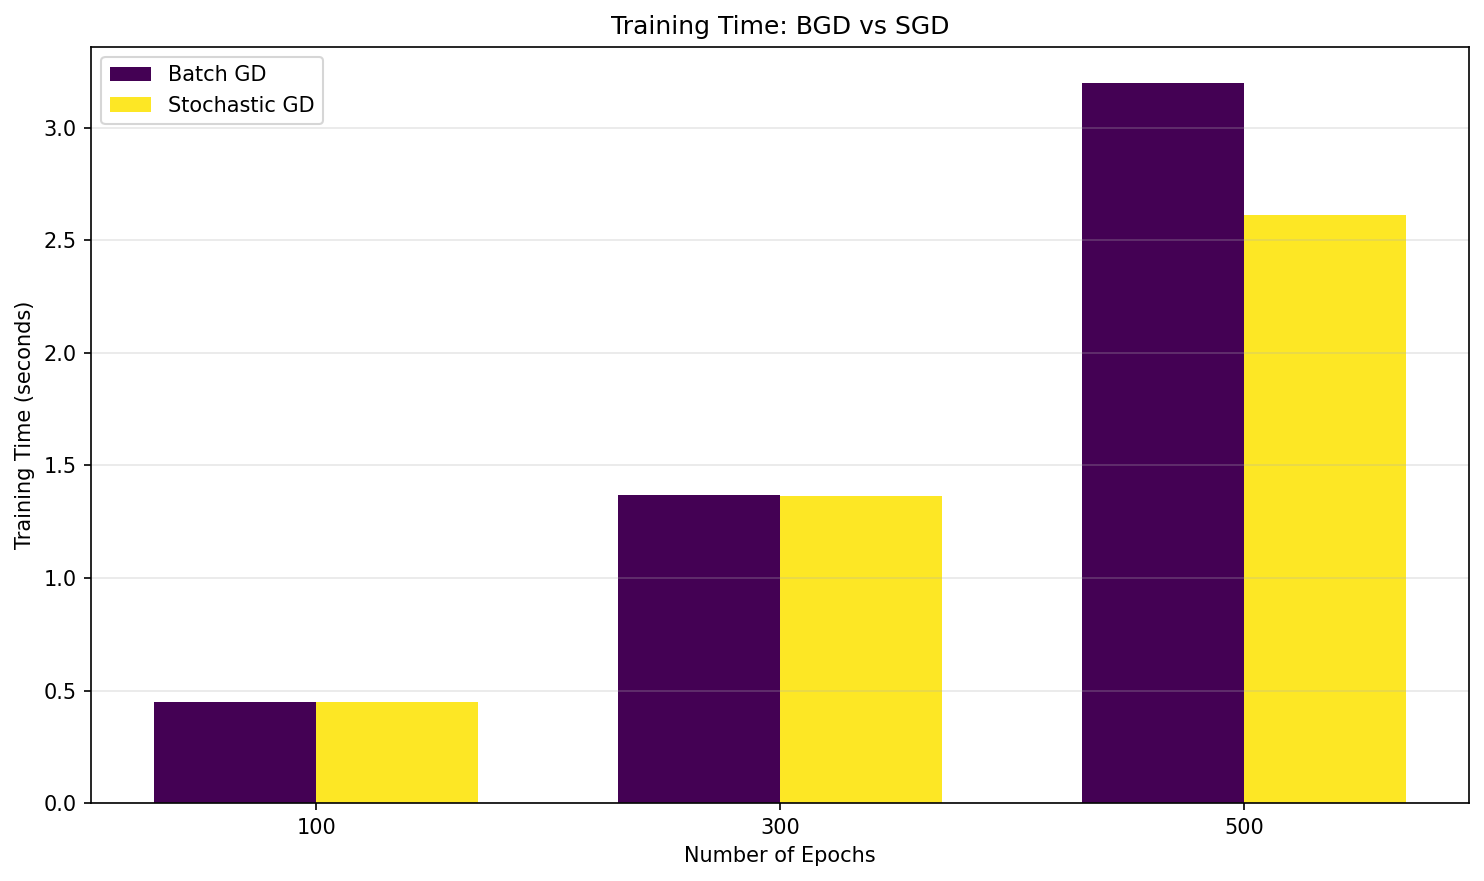
\includegraphics[width=0.85\linewidth]{2Lab/visualizations/time_comparison.png}
    \caption{Mokymo laiko palyginimas esant vienodam epochų skaičiui}
    \label{fig:time_comparison}
\end{figure}

Mokymo laikas abiem metodams yra panašus išskyrus atvejį su $epoch = 500$. Didėjant epochų skaičiui pradeda matytis, jog stochastinis metodas tampa greitesniu, tačiau skirtumas nėra didelis.